\subsection{Gestion d'erreur en C}
  Une partie de cette semaine a été consacrée au débogage du comptage écrit en C. En effet le comptage à la racine avec une fenêtre de 50, provoquait des erreurs 
  d'allocation mémoire. Ce problème fut régler grâce à la re-allocation de la mémoire, moins coûteux que de faire une nouvelle allocation. 
  \subsection{Taille du jeu de fréquences à la racine}
  Avec une taille de fenêtre glissante constante, la taille du fichier de fréquence est proportionnel à la somme des tailles de séquences (nombre de nucléotides totale). On a pu évaluer ainsi la taille du fichier de fréquence au plus haut niveau avec une fenêtre de taille 50 et le pattern \#\#\#\#. On obtiendrai au niveau de la racine, une taille de \textbf{123Go} pour le fichier de fréquence et un temps de \textbf{120 min}. Ainsi grâce aux graphes ci dessous on a pu évaluer le temps (fig. \ref{temps_cpt}) pour générer le fichier de fréquence et la taille de celui-ci (fig. \ref{taille_cpt}) sur l'ensemble des séquences (251 371 097 nucléotides).
  
  
\begin{figure}[H]
\begin{center}
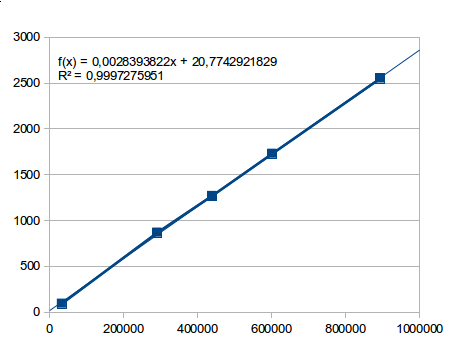
\includegraphics[scale=0.6]{./../img/graphe_temps.png}
\caption[Temps de du comptage]{\label{temps_cpt}Temps en seconde en fonction de la taille de la séquence avec une fenêtre de taille 50}
\end{center}
\end{figure}

\begin{figure}[H]
\begin{center}
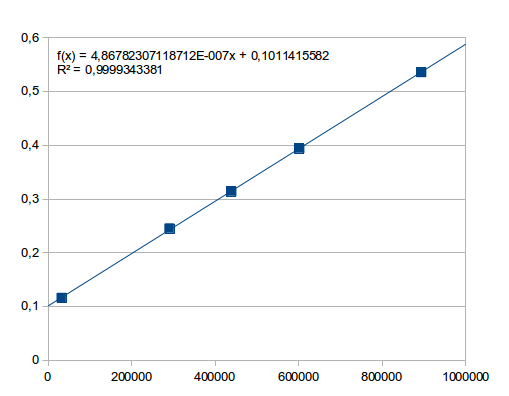
\includegraphics[scale=0.6]{./../img/graphe_taille.png}
\caption[Temps de du comptage]{\label{taille_cpt}Temps en seconde en fonction de la taille de la séquence avec une fenêtre de taille 50}
\end{center}
\end{figure}
  
\subsection{Passage aux objets}
Pour la suite du projet on décide de passer au c++ afin de tout gérer en tant qu'objet, on pourra ainsi plus aisément manipuler la table de fréquence en kmers. La génération
de données pour weka, la validation croisée (avec les cartes...) ...
\subsubsection{Les classes}
Pour le moment on ne manipule que trois classes:
\begin{itemize}
 \item classData: pour gérer les données (séquences,taille, nombre de jeux de données, responsable du comptage)
  \item classPattern: gestion d'un kmer
  \item FreqKmer: classe principale gérant principalement le tableau de fréquence.
\end{itemize}
~\\

L'objet à la possibilité de s'instancier à partir 
\begin{itemize}
 \item[.] D'un fichier fasta
 \item[.] D'un fichier contenant une liste de chemins vers des fichiers fasta.
\end{itemize}
~\\

De ce fait lorsqu'on souhaite obtenir la fréquence à un niveau, c'est au niveau des feuilles du sous arbre définit par ce niveau où l'on va effectuer le comptage.

En fin de semaine des tests de validation ont été rajoutés au programme. Le programme est fonctionnel et les tests le confirment.
